\section{Physical View}
\label{sec:PhysView}

\subsection{Release}
\label{subsec:Release}

Because this project was made in unity, it utilizes a file made by unity to handle crashes.
This file is called Unity \textit{UnityCrashHandler64.exe} within the file system.

When downloading the release version from the Github repository previously mentioned in \ref{subsec:BackgroundInfo}, the build is downloaded as a zip file.
When unzipped, there lies the Crash Handler from Unity alongside the exe file to run the game.
The .exe file to run the game is called \textit{MineSweeper.exe}.

The zipped folder is 39MB large.
When unzipped, the size grows to 81MB.

If any bug fixes should occur, then by releasing the changes under the main branch, I will be able to pull the changes on the release branch.
From the release branch, I can release the update so that people wanting to download the new version are able to.

Because I am not monetizing this project, I don't expect legal issues.
If required I can also utilize a License for distribution to overcome such issues.

\subsection{Unity Editor View}
\label{subsec:UEView}

The Unity Editor was a powerful tool for connecting the scripts to the visual elements within the game space that would be presented to the player visually.
It was nice not having to worry about effects such as light, reflections, collision, and other components typically used in games.
The exclusion of such components was because they were deemed unnecessary.

\begin{figure}[!htpb]
    \centering
    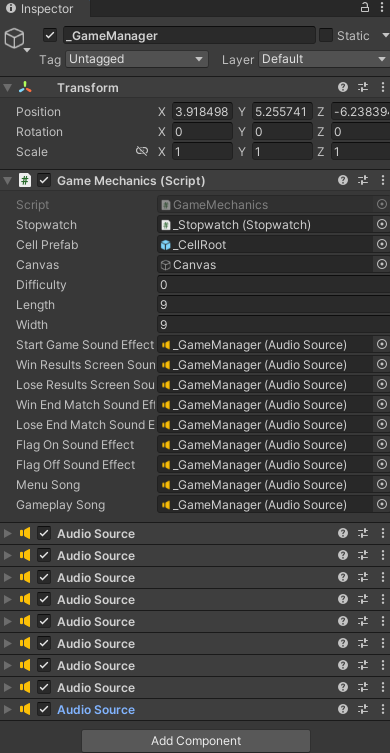
\includegraphics[width=10cm]{Images/UEViewGM.png}
       \caption{What the object \textit{\_GameMechanics} looks like in the Unity Editor.}
           \label{Fig:UEViewGM}
\end{figure}

